\section{Wzorce projektowe (1) - konstrukcyjne}
\url{https://softwareengineering.stackexchange.com/questions/365119/is-using-new-in-the-constructor-always-bad}
Wzorce kreacyjne pozwalają na tworzenie obiektów w sposób zwiększający elastyczność. Zamiast tworzyć obiekty w wielu miejscach w programie, zadaniem konstrukcji nowych instancji można obciążyć osobne klasy. Użycie słowa kluczowego \texttt{new} narusza omawianą wcześniej zasadę odwracania zależności, powodując trudności z testowaniem kodu i zmniejszając jego elastyczność. 

\subsection{Fabryka abstrakcyjna (ang. abstract factory)}
Fabryka abstrakcyjna jest wzorcem projektowym, który przenosi proces tworzenia obiektów (często ze sobą w jakiś sposób powiązany) do osobnej klasy implementującej interfejs zawierający listę metod tworzących dane obiekty. Co więcej tworzone przez fabryki instancje również powinny posiadać zgodne interfejsy.

Klient może posiadać konstruktor, który jako parametr przyjmie obiekt implementujący interfejs abstrakcyjny. Wewnątrz konstruktora klient wywołując odpowiednie metody może tworzyć konkretne obiekty bez znajomości ich szczegółowej implementacji. Przekazując inny obiekt fabryki abstrakcyjnej możliwa jest łatwa zmiana wykorzystywanych przez klienta obiektów.  

Przykład:
Aplikacja wykorzystująca interfejs graficzny mogłaby przyjmować jako argument obiekty fabryki implementujące interfejs \texttt{IGuiFactory}. Interfejs ten mógłby definiować metody tworzenia poszczególnych elementów graficznych np. \texttt{createButton()}, \texttt{createListBox()}, \texttt{createProgressBar()} itp. Następnie w zależności od systemu operacyjnego można by stworzyć obiekty fabryk \texttt{WindowsFactory} oraz \texttt{UnixFactory}, oba implementujące określony wcześniej interfejs. Aplikacja posiadające logikę rysująca okno użytkownika nie musi w takim przypadku nawet wiedzieć z jakim systemem ma do czynienia, jest od niego niezależna. Może wywoływać metody tworzące kontrolki UI za pomocą abstrakcyjnego interfejsu \texttt{IGuiFactory}. Wybór konkretnej fabryki mógłby być określany w momencie uruchamiania się aplikacji.



\begin{figure}[hbt!]
	\centering
	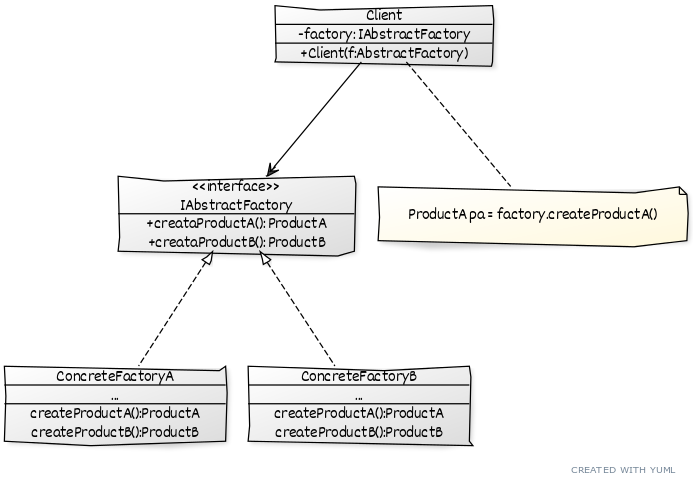
\includegraphics[width=0.9\linewidth]{images/AbstractFactoryUml}
	\caption{Diagram UML wzorca Fabryka Abstrakcyjna.}
	\label{lab2/fig/AbstractFactoryUml}
\end{figure}
%[Client]->[IAbstractFactory]
%[Client]-[note: ProductA pa = factory.createProductA(){bg:cornsilk}]
%[IAbstractFactory]^-.-[ConcreteFactoryA]
%[IAbstractFactory]^-.-[ConcreteFactoryB]
%
%[≪interface≫;IAbstractFactory|+creataProductA(): ProductA;+creataProductB(): ProductB;]
%[Client|-factory: IAbstractFactory|+Client(f:AbstractFactory);]
%[ConcreteFactoryA|...|createProductA():ProductA;createProductB():ProductB]
%[ConcreteFactoryB|...|createProductA():ProductA;createProductB():ProductB]


\subsection{Budowniczny (ang. builder)}
Budowniczy jest wzorcem, który może być wykorzystany do tworzenia złożonego obiektu krok po kroku. Czasami istnieje pokusa stworzenia konstruktora przyjmującego dużą liczbę argumentów np. dana klasa korzysta z wielu zależności albo niektóre jej cechy mogą być parametryzowane. Część z tych argumentów może w ogóle nie być konieczna. Budowniczy przenosi proces tworzenia takiej instancji do osobnego obiektu. 

Czynności wywoływania poszczególnych metod można przenieść do osobnego obiektu kierownika (ang. director), który będzie przyjmował jako argument konstruktora obiekt budowniczego i wywoływał metody interfejsu \texttt{IBuilder}.

Konkretni budowniczowie powinni dostarczyć swoje własne metody zwracania wyników procesu budowania obiektu. Różni budowniczowie mogą zwracać zupełnie inne typy dlatego tego procesu często nie da się umieścić w interfejsie \texttt{IBuilder} (przynajmniej w przypadku języków programowania, które są silnie typowane). 
 
Wzorzec budowniczy często wspiera tzw. płynne interfejsy (ang. Fluent Interface). Z przykładem użycia tego mechanizmu można się spotkać w zapytaniach LINQ, gdzie zamiast wywoływać kolejne metody progresywnie (w kolejnych wierszach), można je wywoływać kaskadowo po kropce.

\begin{lstlisting}[caption={Wykorzystanie płynnych interfejsów w zapytania LINQ}, label={lab2/lst/fluentInterfaceLinq}]
var translations = new Dictionary<string, string>
{
	{"cat", "chat"},
	{"dog", "chien"},
	{"fish", "poisson"},
	{"bird", "oiseau"}
};

// Find translations for English words containing the letter "a",
// sorted by length and displayed in uppercase
IEnumerable<string> query = translations
.Where   (t => t.Key.Contains("a"))
.OrderBy (t => t.Value.Length)
.Select  (t => t.Value.ToUpper());

// The same query constructed progressively:
var filtered   = translations.Where (t => t.Key.Contains("a"));
var sorted     = filtered.OrderBy   (t => t.Value.Length);
var finalQuery = sorted.Select      (t => t.Value.ToUpper());
\end{lstlisting}

W przeciwieństwie do wzorca fabryki abstrakcyjnej, która tworzy obiekty (często ze sobą powiązane) w jednym kroku, budowniczy tworzy jeden złożony obiekt krok po kroku.